% ****** Start of file apssamp.tex ******
%
%   This file is part of the APS files in the REVTeX 4.2 distribution.
%   Version 4.2a of REVTeX, December 2014
%
%   Copyright (c) 2014 The American Physical Society.
%
%   See the REVTeX 4 README file for restrictions and more information.
%
% TeX'ing this file requires that you have AMS-LaTeX 2.0 installed
% as well as the rest of the prerequisites for REVTeX 4.2
%https://www.overleaf.com/project/6013d24d3206742babfa0cac% See the REVTeX 4 README file
% It also requires running BibTeX. The commands are as follows:
%
%  1)  latex apssamp.tex
%  2)  bibtex apssamp
%  3)  latex apssamp.tex
%  4)  latex apssamp.tex
%
\documentclass[%
 reprint,
%superscriptaddress,
%groupedaddress,
%unsortedaddress,
%runinaddress,
%frontmatterverbose, 
%preprint,
%preprintnumbers,
%nofootinbib,
%nobibnotes,
%bibnotes,
 amsmath,amssymb,
 aps,
%pra,
%prb,
%rmp,
%prstab,
%prstper,
%floatfix,
]{revtex4-2}

\usepackage{graphicx}% Include figure files
\usepackage{dcolumn}% Align table columns on decimal point
\usepackage{bm}% bold math
\usepackage{minted}
%\usepackage{hyperref}% add hypertext capabilities
%\usepackage[mathlines]{lineno}% Enable numbering of text and display math
%\linenumbers\relax % Commence numbering lines

%\usepackage[showframe,%Uncomment any one of the following lines to test 
%%scale=0.7, marginratio={1:1, 2:3}, ignoreall,% default settings
%%text={7in,10in},centering,
%%margin=1.5in,
%%total={6.5in,8.75in}, top=1.2in, left=0.9in, includefoot,
%%height=10in,a5paper,hmargin={3cm,0.8in},
%]{geometry}

\begin{document} 

\preprint{APS/123-QED}

\title{Inertial Measurement Unit with Applications}% Force line breaks with \\
%\thanks{A footnote to the article title}%

\author{Six Flags (Xinyuan Lin, Jichen Zhang, \AE ther Zhou)}


\begin{abstract}
Inertial Measurement Unit (IMU) is widely used in our daily electric devices, such as cell phone and tablet. A typical IMU consists of accelerometers and gyroscopes. It can read 3 axis’ linear acceleration and angular velocity. In this project, we used ISM330DHCX – 6 DoF IMU with Raspberry Pi to collect raw data. Then we applied IMU sensor fusion algorithm to calculate the absolute rotation with to convert accelerations. At the end, we attempted to integrate the calibrated acceleration twice to find the displacement. We tested our method in different settings. The 1D results is promising with proper filter applied. However, the 3D path is suffering from large noise and low sampling rate. 
% \begin{description}
% \item[Usage]
% Secondary publications and information retrieval purposes.
% \item[Structure]
% You may use the \texttt{description} environment to structure your abstract;
% use the optional argument of the \verb+\item+ command to give the category of each item. 
% \end{description}
\end{abstract}

%\keywords{Suggested keywords}%Use showkeys class option if keyword
                              %display desired
\maketitle

%\tableofcontents

\section{Introduction}
From the introductory Newtonian physics class, we have learned that acceleration is the second time derivative of displacement. Theoretically, if we assume the initial position and velocity, we should be able to find the path from the acceleration measurement. 

Inertial Measurement Unit (IMU) has been widely used in measuring acceleration and angular velocity. Most IMU chips in the market use the internal spring-like structure to measure the change in capacitance caused by acceleration and use the similar change in capacitance measurement to calculate angular velocity by Coriolis effect.\cite{structure}

IMU can be found in many devices, cell phones, tablets, smart watch, and even headphones. We have seen data leak event\cite{news} on news all the time, which lead us to wondering if the IMU can be a risk of leaking our personal daily activity log? To what extend such IMU data can be used to track the movement without GPS?

Many previous attempts of building an IMU only used acceleration in one direction.\cite{rpimu} In this project, we extended one dimensional movement to three dimensional movement. We used the Attitude and Heading Reference System (AHRS) algorithm to convert the raw acceleration collected by the accelerator to absolute acceleration. We used ST ISM330DHCX, an industrial quality Accelerometer + Gyroscope 6-DOF IMU from ST and Raspberry Pi 4.   
The hardware is introduced in Section~\ref{Method}. 1D experiment is discussed in Section~\ref{1Dexperiment}. 3D experiment is discussed in Section~\ref{3Dexperiment}. And Section~\ref{Discussion} is discussion.


\section{\label{Method}Method}
We used Adafruit ISM330DHCX\cite{ism} - 6 DoF IMU - Accelerometer and Gyroscope as our sensor. It can measure ±2/±4/±8/±16g and ±125/±250/±500/±1000/±2000/±4000 degree per second up to 6.7 KHz update rate.
\begin{figure}[H]
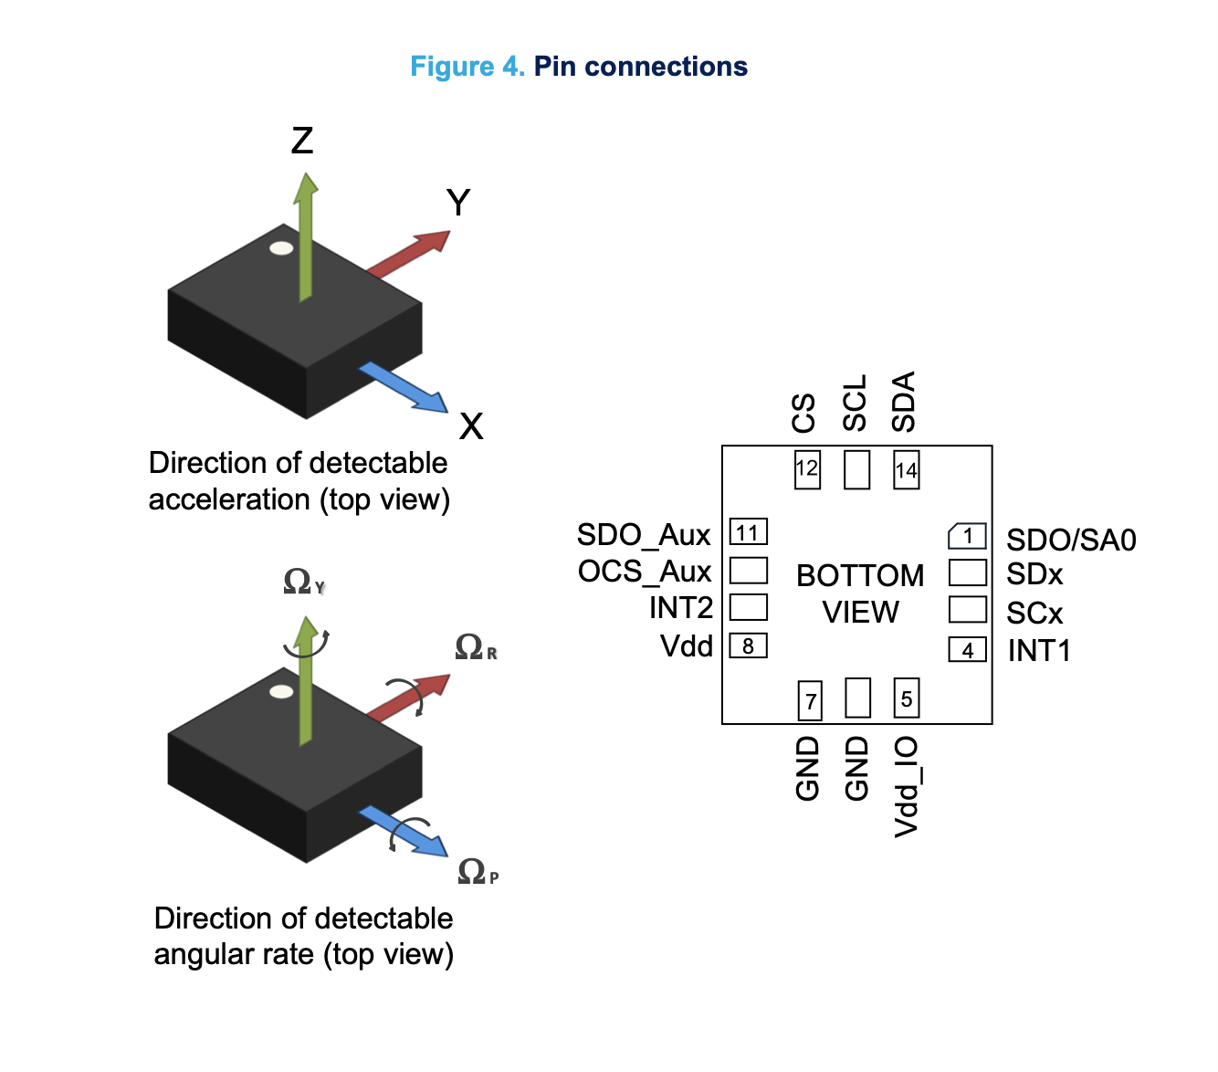
\includegraphics[width=0.5\textwidth]{sensor.png}
\caption{\label{superman}How the motion data is measured.}
\end{figure}

The IMU is connected to a Raspberry Pi via cables. It is also powered by Raspberry Pi with 5V output. The Raspberry Pi is powered by a normal power bank via USB type-C cable. We initially used Raspberry Pi Pico\cite{pico} for 1D experiment, then we switched to Raspberry Pi 4 to increase the sampling rate. I2C protocol\cite{i2c} is used by Raspberry Pi to read data from the IMU. The python code for Pi is attached in appendix.

For Raspberry Pi Pico, we programmed it as when power is plugged in, run the program to collect data for the time we defined. We used the LED on the Raspberry Pi Pico to indicate if the data collection has started or ended.

For Raspberry Pi 4\cite{pi4}, we need to use Wi-Fi to control it. In our experiment, we find that iPhone’s hotspot is not very stable and sometime can unexpectedly disconnect. Since we are using ssh to control the Raspberry Pi 4, a disconnection in network will interrupt the data collection. After different attempts, we find a solution. We using iPhone A as the hotspot. Then let Raspberry Pi 4 and iPhone B to connect to it. We used iPhone B to ssh to Raspberry Pi 4 to control the data collection.
\begin{figure}[H]
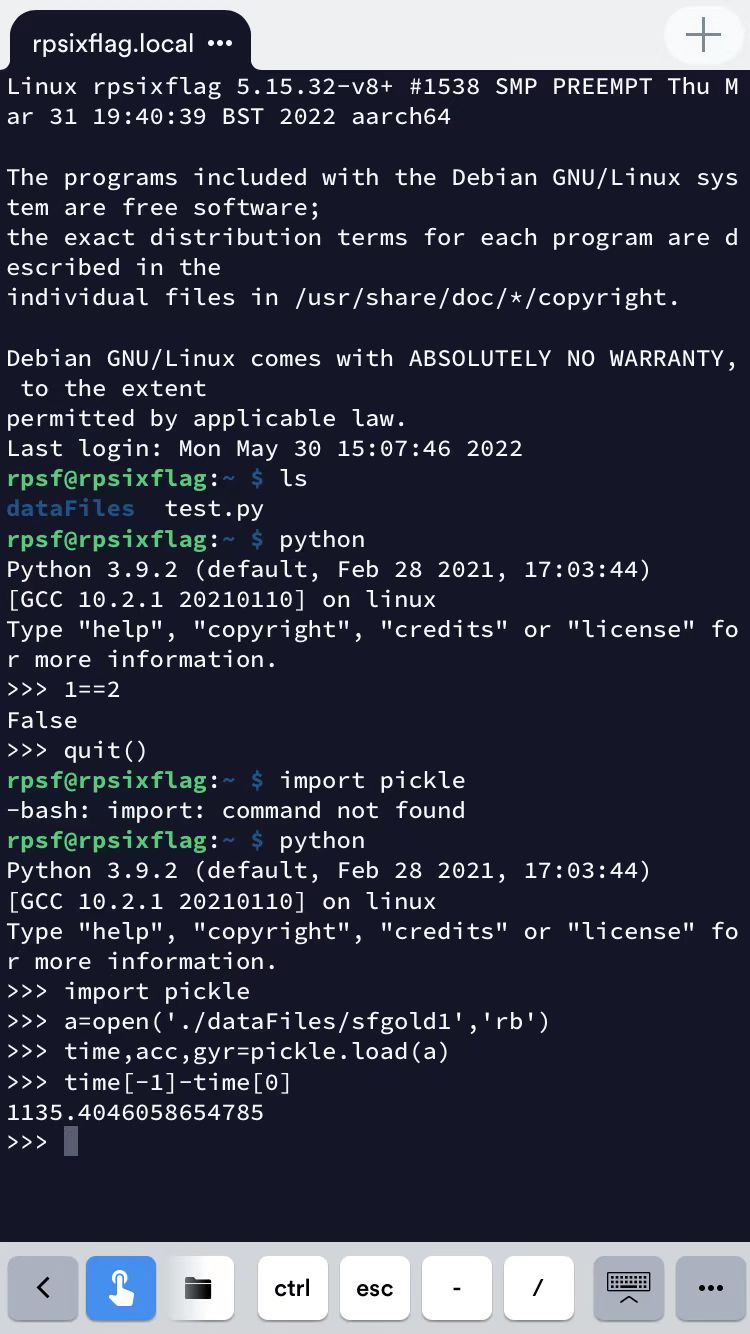
\includegraphics[width=0.12\textwidth]{ssh.jpg}
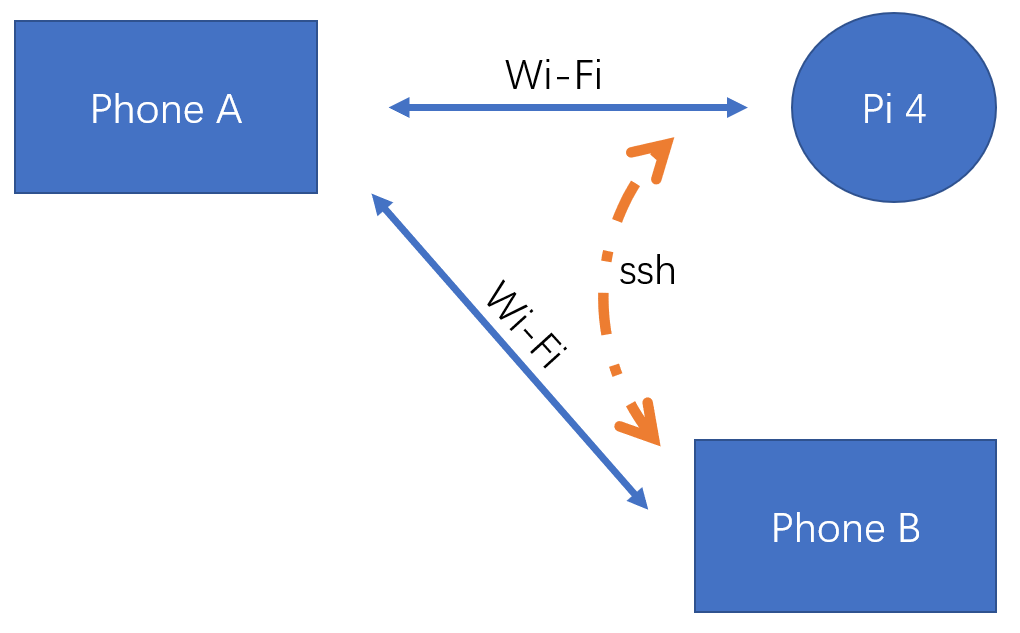
\includegraphics[width=0.38\textwidth]{ssh2.png}
\caption{\label{superman}SSH connection via Wi-Fi.}
\end{figure}

The raw data is saved as a .csv file. Each row has the time interval, 3 linear acceleration on $x, y, z$ axis in m/s$^2$, and 3 angular velocity in degree/s. Note that the raw data has gravity included, which need to be subtracted in data processing.

\section{\label{1Dexperiment}1D Experiment}
We take our device to the elevator to conduct experiment for 1 dimensional movement. In this experiment, we only take the movement in Z-axis into account. The result is presented in the figure.

We found that if we simply integrate the raw data twice, the displacement does not reflect the true movement. However, we add a filter on the velocity before second integration, which improved our result to a more realistic movement. The filter is a cut off the lower velocity, which we considered as vibration. However, if the threshold is too high, we are losing the precision of our measurements due to the ignorance of the low speed of the movement. Based on the comparison showed in the figure, 0.004 m/s is an optimized threshold value for the filter. Based on this experiment, we found the average height of Broida building is about 3.5 meter. 
\begin{figure}[H]
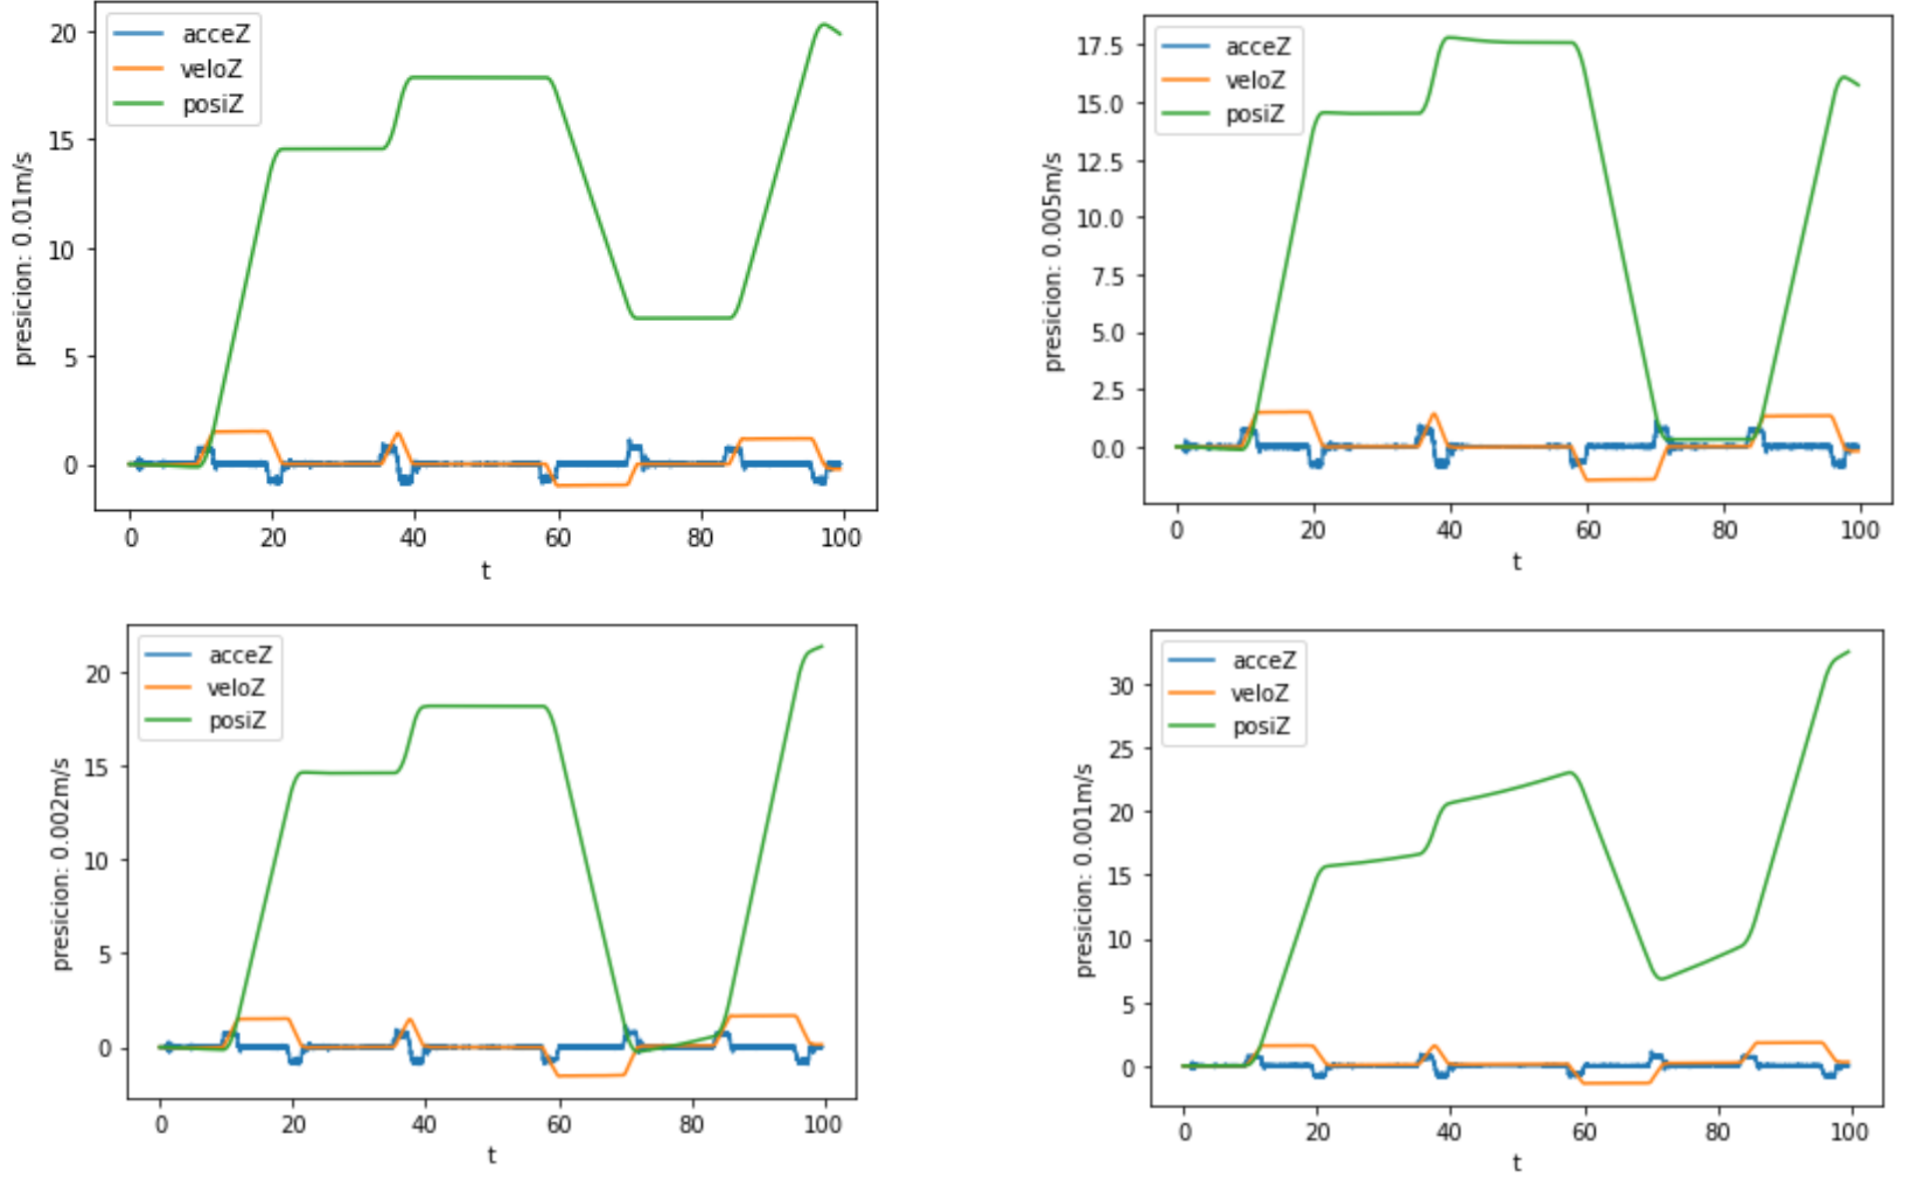
\includegraphics[width=0.48\textwidth]{broida.png}
\caption{\label{broida}Integrated result from experiment in Broida hall elevator.}
\end{figure}

\section{\label{3Dexperiment}3D Experiment}
In order to measure the 3D movement, we need to use fusion algorithm to covert the 6 DoF data we have to absolute rotation and acceleration data.
\begin{figure}[H]
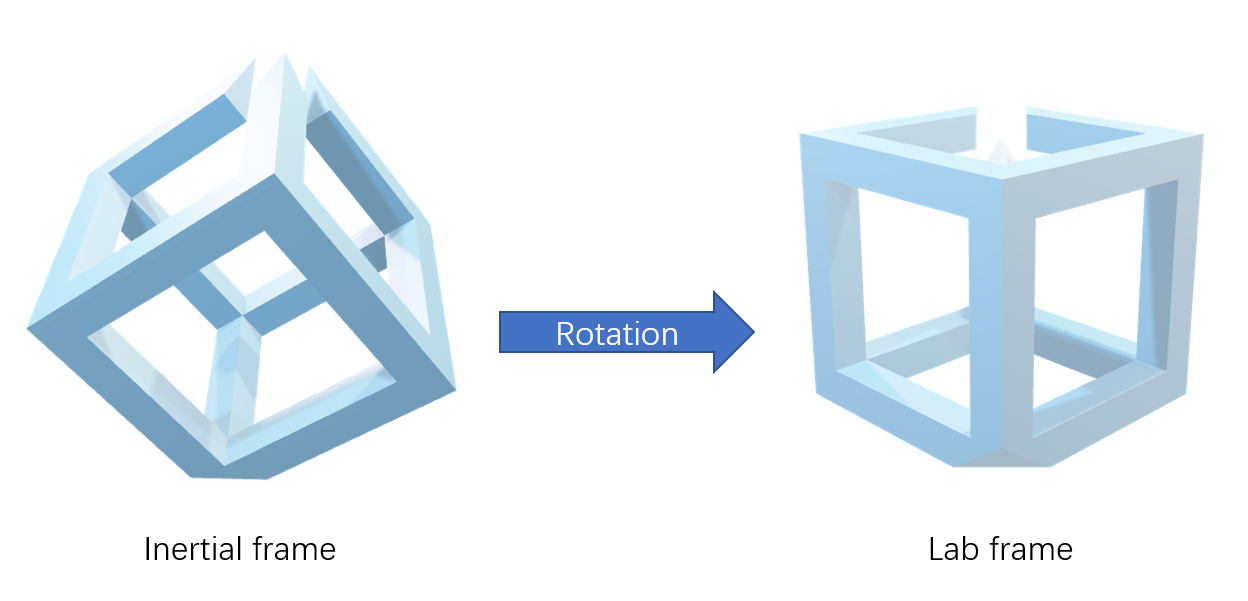
\includegraphics[width=0.4\textwidth]{rotation2.png}
\caption{\label{rotation2}Transform the raw data in rotated frame into lab frame.}
\end{figure}

\subsection{IMU fusion algorithm}
We used a python library that used Attitude and Heading Reference System (AHRS)\cite{ahrs,ahrsthesis} algorithm combines our raw data. It gives the Euler angles. We then use the Euler angles to rotate the raw acceleration to find the absolute acceleration. Code showed in Appendix~\ref{Code}.

\newpage

\subsection{Test on Rotation}
We did an experiment to test the algorithm by only rotate our device, the result matches the movement we applied, see Figure~\ref{rotation}. 

\begin{figure}[H]
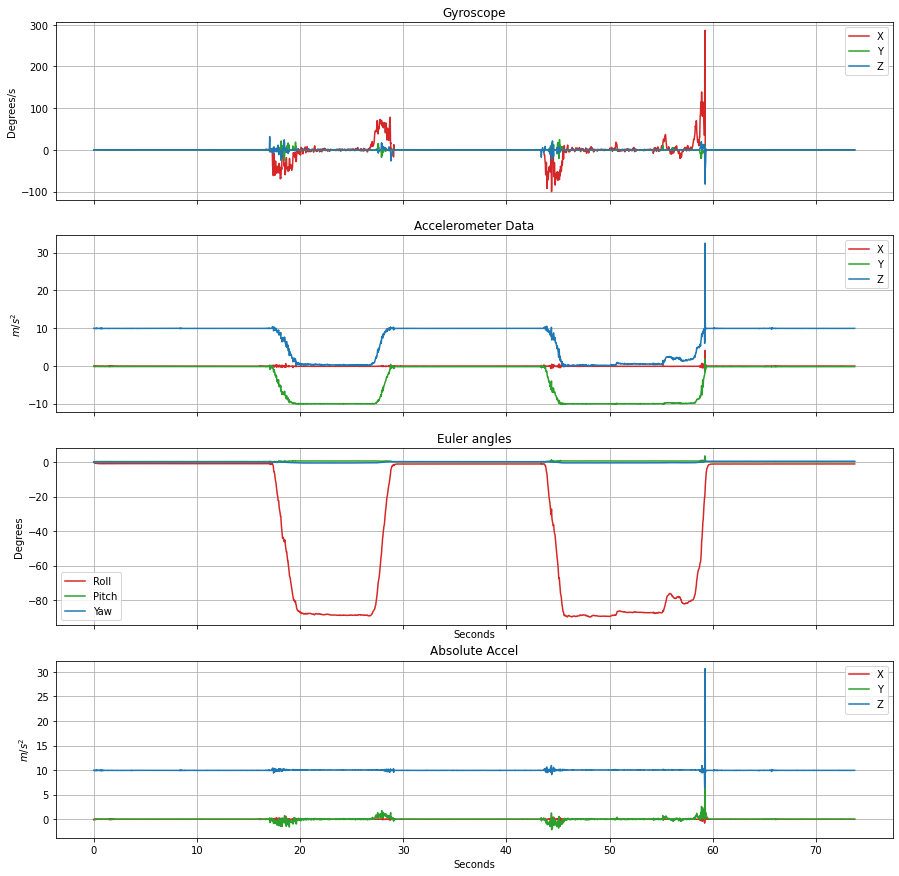
\includegraphics[width=0.48\textwidth]{rotation.png}
\caption{\label{rotation}In this test, we rotated our device around $x$ axis by 90 degrees, which was shown in the plot.}
\end{figure}

\subsection{Merry-Go-Round}
We did an experiment to test the algorithm by only rotate our device, the result matches the movement we applied, see Figure~\ref{mgr}.

The path indicated a circular motion, which is very close to the actual movement. The period is about 2 mins.
\begin{figure}[H]
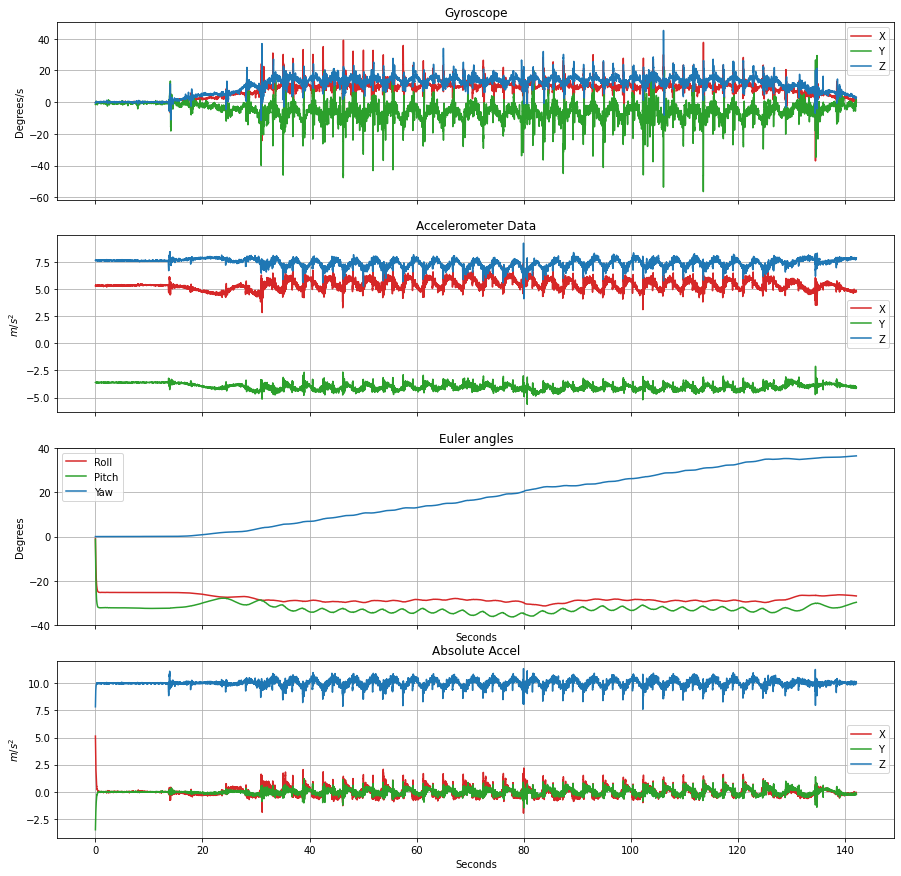
\includegraphics[width=0.48\textwidth]{mgr.png}
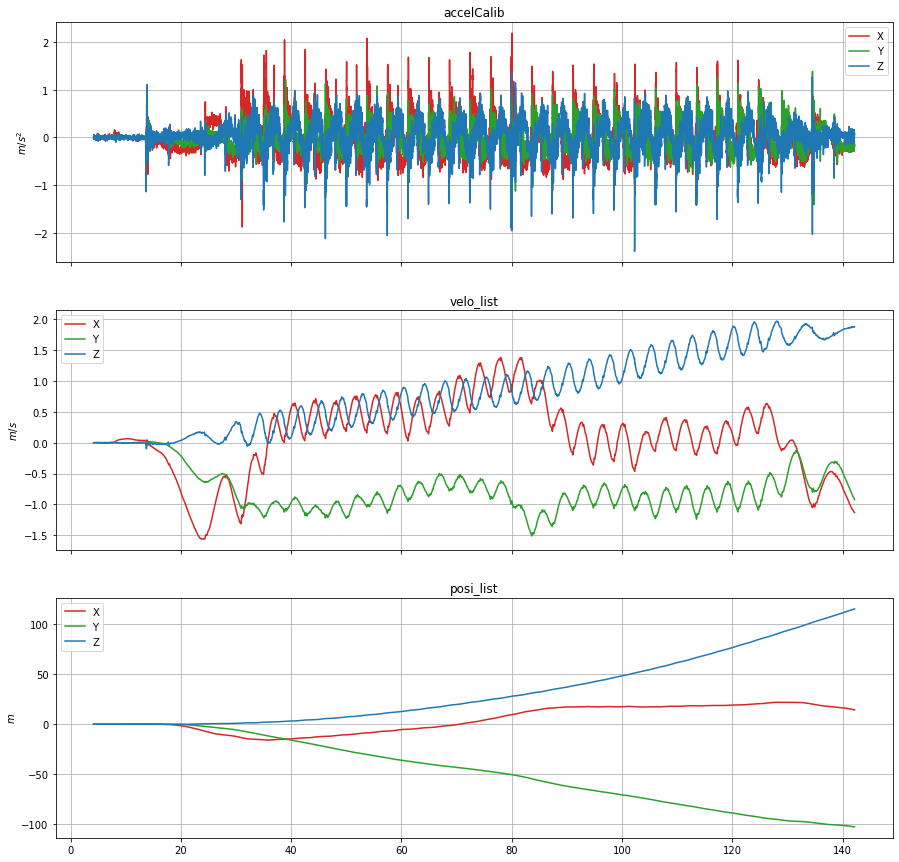
\includegraphics[width=0.48\textwidth]{mgr_integrate.png}
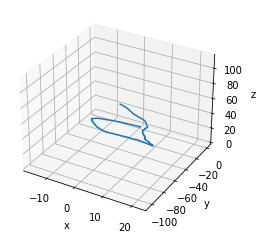
\includegraphics[width=0.35\textwidth]{mgr_path.png}
\caption{\label{mgr}Merry-Go-Round.}
\end{figure}


\subsection{Superman}
Superman is a ride in Six Flags\cite{sixflags} that with a simple path. It accelerates horizontally to over 100 mph and the track become vertical and does the free fall. Our measurement can clearly see the change in acceleration. It clearly shows the 1 g free fall and the two symmetrical centripetal acceleration when the car turning between the horizontal track and vertical track. However, due to the large noise from vibration, the integrated result is not satisfying.




\subsection{Viper}
Six Flags Viper has all kinds of movement for a roller coaster. The track is complex and long. Luckily, we did two trials to for this ride. The results show some similarity (see Figure~\ref{viper1} and Figure~\ref{viper2}) but the large noise makes the integrated result not reliable.

\section{\label{Discussion}Discussion}
Our project shows a method to use a common IMU to make measurement for displacement. The 1D experiment with filter shows promising results, but 3D data still suffer from large noise. We attempted use existed noise reduction package to reduce the noise, but the result doesn't have significant change. We find that even the IMU has 6.6KHz update rate, our actual rate is about 250 Hz. We believe this is limited by the bandwidth of Raspberry Pi and the I2C protocol. We tried to use SPI protocol\cite{spi} to save the bandwidth so we can have a higher sampling rate. However, the package provided by Adafruit for this IMU for SPI protocol only works on Arduino. It was too late to switch our platform. The lesson learnt here is try to keep use the same platform with the preexisted package. If we can have a higher sampling rate, the noise will be smoothed, and the vibration will not affect too much on the final results. 

This finding shows that with low sampling rate, it is not easy to calculate the path based on the IMU raw data. This can be a big relive. If your cell phone are collecting IMU data at high rate, the battery will shortly dies out and you will notice it. Therefore, we don’t really need to worry too much about it.

\begin{figure}[H]
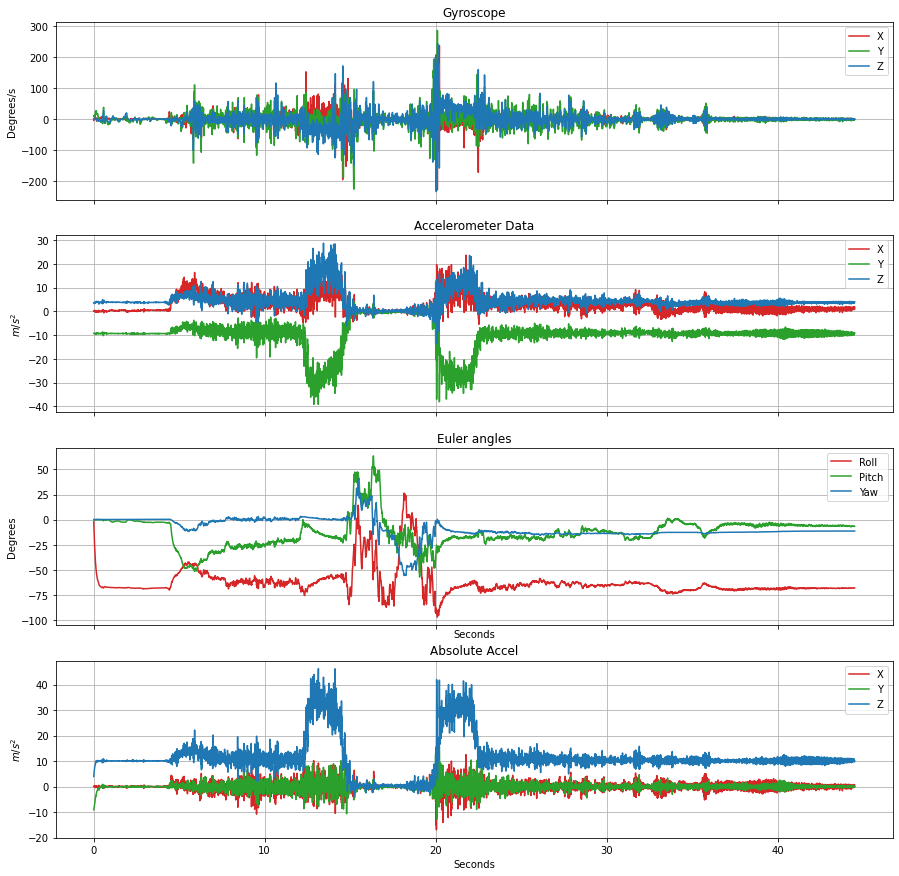
\includegraphics[width=0.48\textwidth]{superman.png}
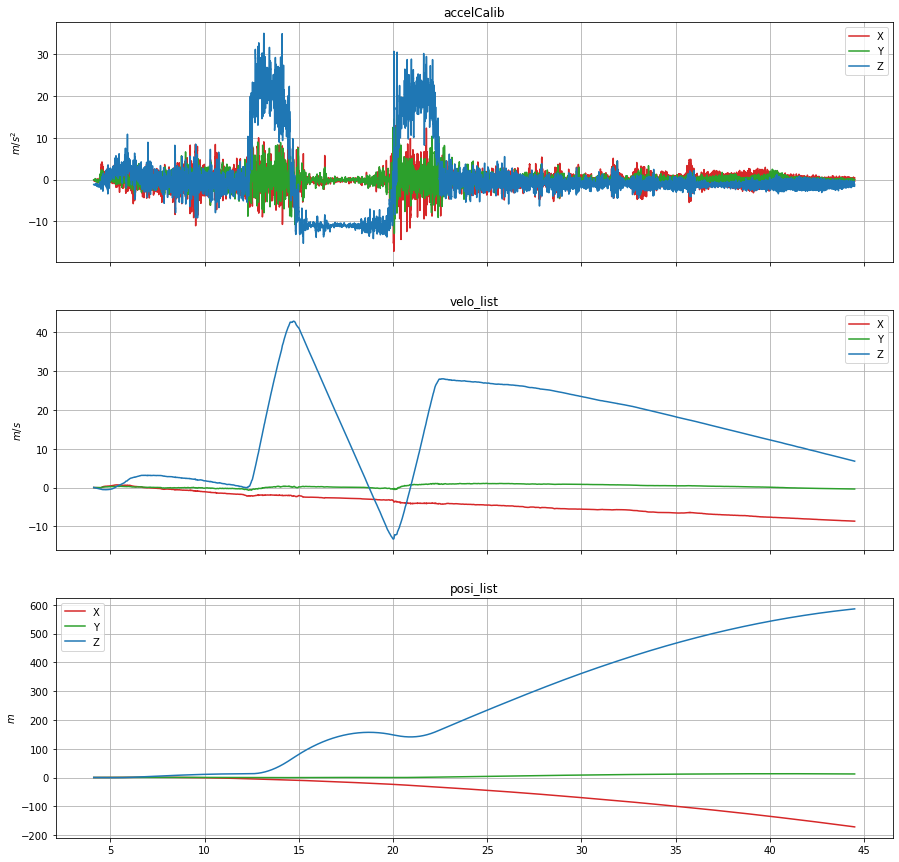
\includegraphics[width=0.48\textwidth]{superman_integrate.png}
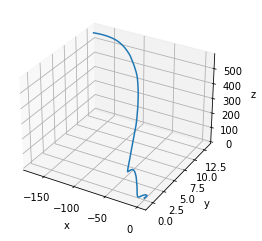
\includegraphics[width=0.35\textwidth]{superman_path.png}
\caption{\label{superman}Superman.}
\end{figure}


\begin{figure}[h]
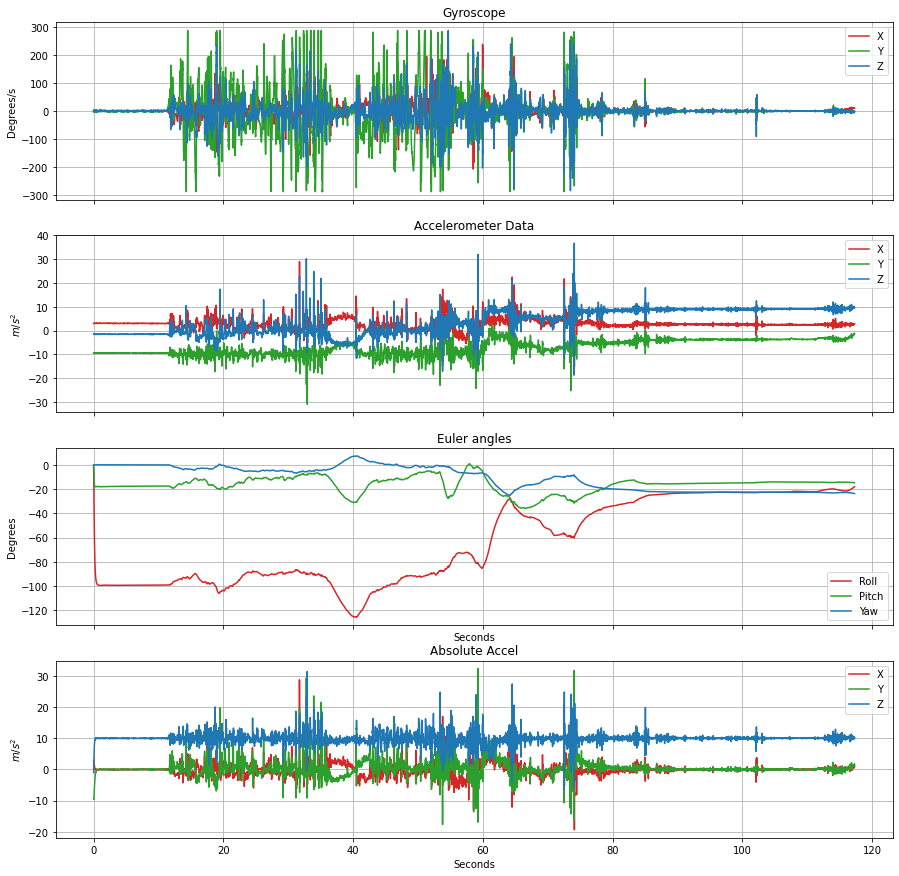
\includegraphics[width=0.48\textwidth]{viper1.png}
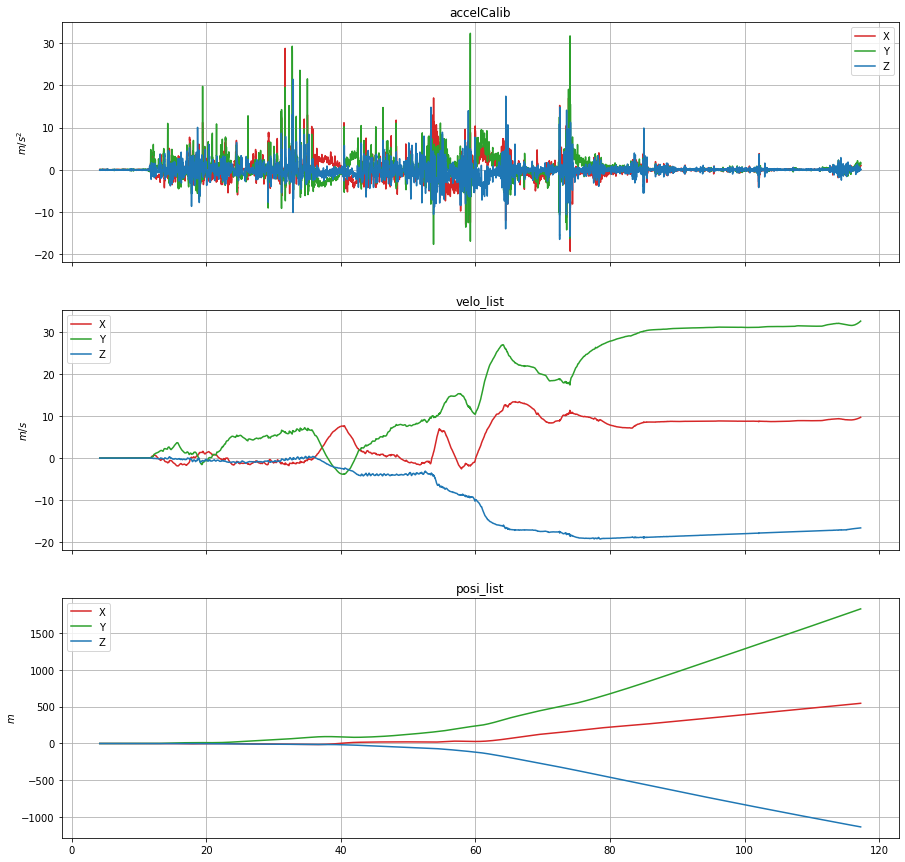
\includegraphics[width=0.48\textwidth]{viper1_integrate.png}
\caption{\label{viper1}The first ride of Viper.}
\end{figure}

\begin{figure}[h]
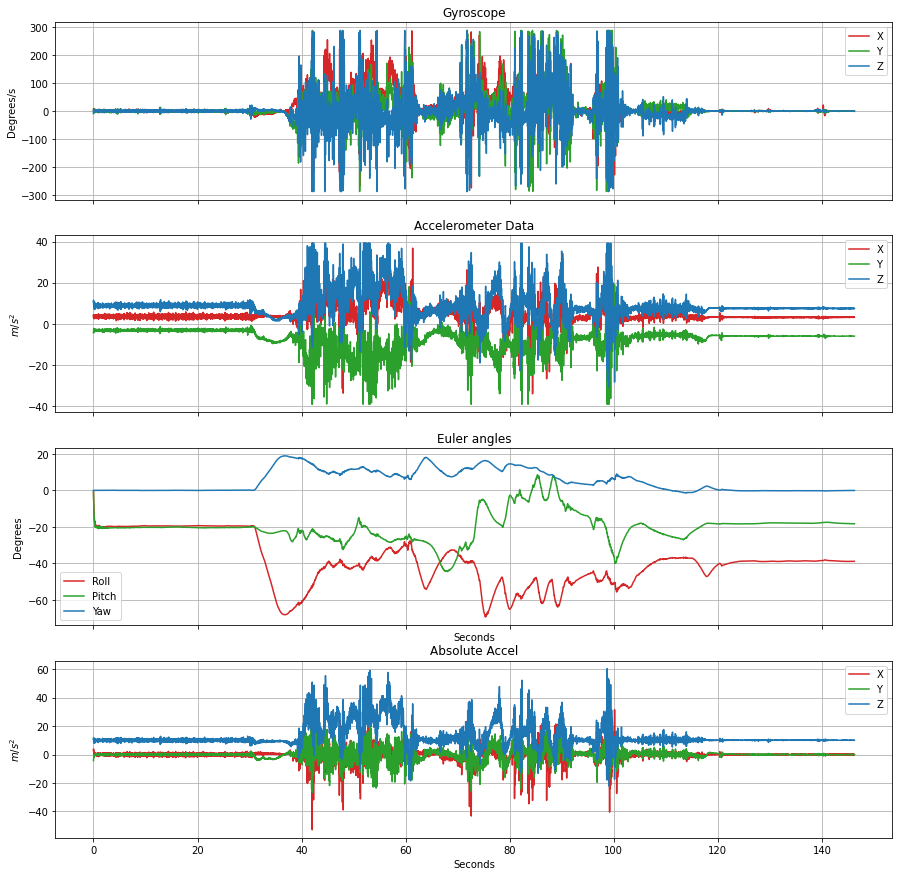
\includegraphics[width=0.48\textwidth]{viper2.png}
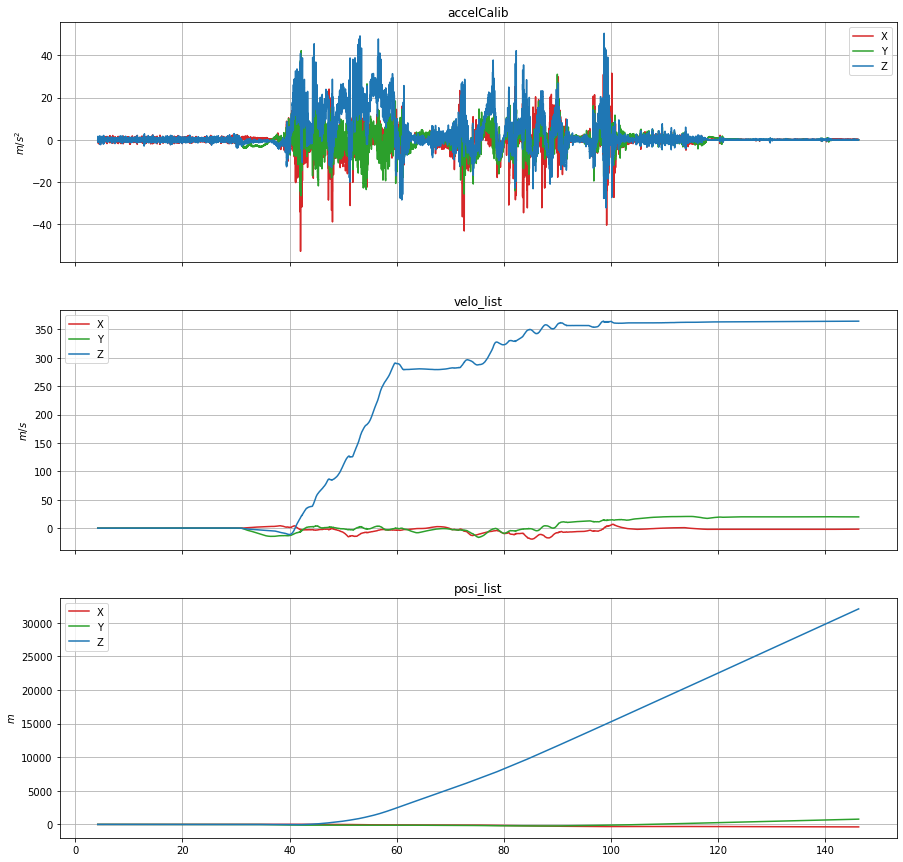
\includegraphics[width=0.48\textwidth]{viper2_integrate.png}
\caption{\label{viper2}The second ride of Viper.}
\end{figure}


\appendix

\section{\label{Code}Data Analysis Scripts}

\begin{minted}[breaklines]{python}
"""
@author: Six Flags (Xinyuan Lin, Jichen Zhang, Bangda Zhou)
"""
import numpy as np
import imufusion
from scipy.spatial.transform import Rotation as R
import matplotlib.pyplot as plt
import pickle

def get_data(fileName):
    my_Data = open(fileName, 'rb')
    timeLog,acceLog,gyroLog= pickle.load(my_Data)
    my_Data.close()
    t_interval_list = [0]
    accel_3d_list = [[acceLog[0][0], acceLog[0][1], acceLog[0][2]]]
    omega_3d_list = [[gyroLog[0][0], gyroLog[0][1], gyroLog[0][2]]]
    for i in range(len(timeLog)-1):
        t_interval_list.append(timeLog[i+1] - timeLog[i])
        accel_3d_list.append([acceLog[i+1][0], acceLog[i+1][1], acceLog[i+1][2]])
        omega_3d_list.append([gyroLog[i+1][0], gyroLog[i+1][1], gyroLog[i+1][2]])
    return np.array(t_interval_list), np.array(accel_3d_list), np.array(omega_3d_list)

def get_timelist(time_interval_list):
    tot_num = len(time_interval_list)
    t_list = [time_interval_list[0]]
    for index in range(1,tot_num,1):
        t_list.append(t_list[index-1] + time_interval_list[index])
    return np.array(t_list)

def calibrator(target_list, t_list):
    index = 1500 # use first 1500 measures to calibrate
    calib_g = sum(target_list[:index])/index
    calibrated_list = target_list - calib_g
    return calibrated_list

def get_1dtraj(accel_list, t_interval_list, threshold=0.004):
    velo_list = [0]
    for index in range(1,len(accel_list),1):
        v = t_interval_list[index] * accel_list[index] + velo_list[index-1]
        if abs(v)<threshold:
            velo_list.append(0)
        else:
            velo_list.append(v)
    velo_list = np.array(velo_list)
    posi_list = [0]
    for index in range(1,len(accel_list),1):
        x = (t_interval_list[index]** 2) * accel_list[index]/2 + velo_list[index] * t_interval_list[index] + posi_list[index-1]
        posi_list.append(x)
    posi_list = np.array(posi_list)
    return velo_list, posi_list

def get_3dAbsAccel(accel_3d_list, omega_3d_list, t_list):
    sample_rate = (t_list[-1]-t_list[0])/len(t_list)
    ahrs = imufusion.Ahrs()
    euler = np.empty((len(t_list), 3)) 
    for index in range(len(t_list)):
        ahrs.update_no_magnetometer( omega_3d_list[index], accel_3d_list[index], sample_rate)
        euler[index] = ahrs.quaternion.to_euler()
        if np.isnan(euler[index][0]):
            euler[index][0] = euler[index-1][0]
        if np.isnan(euler[index][1]):
            euler[index][1] = euler[index-1][1]
        if np.isnan(euler[index][2]):
            euler[index][2] = euler[index-1][2]
    r = R.from_euler('xyz', euler, degrees=True)
    accel_3d_abs_list = r.apply(accel_3d_list)
    return euler, accel_3d_abs_list
\end{minted}


\bibliography{references}% Produces the bibliography via BibTeX.

\end{document}
%
% ****** End of file apssamp.tex ******
